\section{SIFT}
SIFT\footnote{Distinctive Image Features
from Scale-Invariant Keypoints} er en korrespondanceanalyse metode, introduceret af David Lowe i 2004 \cite{SIFT}. SIFT er en samlet løsning, der består af en detektor og en deskriptor.
\subsection{Detektion}
SIFT gør brug af en metode kaldt Difference of Gaussian (DoG), til at finde interessepunkter. DoG er en skala-invariant blob detektor, og er en approksimation til en skalanormaliseret Laplacian of Gaussian (LoG). DoG kan udregnes, ved en subtraktion af et nærliggende skalabillede, separeret af en konstant $k$, hvor $G$ er et Gaussisk filter.
\begin{equation}
\begin{split}
DoG(x,y,\sigma) &= (G(x,y,k\sigma)-(G(x,y,\sigma))\ast I(x,y) \\
           &= L(x,y,k \sigma)-L(x,y,\sigma)
\end{split}
\label{dog}
\end{equation}
Den skalanormaliseret Laplacian of Gaussian kan opstilles som:
\begin{equation}
\begin{split}
LoG(x,y,\sigma)&=\sigma^2\nabla^2L(x,y,\sigma) \\
&= \sigma^2(L_{xx}+L{yy})
\end{split}
\end{equation}
Lowe relatere approksimeringen af DoG til LoG, ved diffusions ligningen:
\begin{equation}
\dfrac{\partial L}{\partial \sigma} = \sigma \nabla^2L
\label{heat}
\end{equation}
Ligning \eqref{heat} kan approksimeres til:
\begin{equation}
\sigma \nabla^2L \approx \frac{G(x,y,k\sigma) - G(x,y,\sigma)}{k\sigma-\sigma}
\label{omskriv}
\end{equation}
Omskrivning af ligning \eqref{omskriv} giver:
\begin{equation}
\begin{split}
(k\sigma-\sigma)\sigma\nabla^2L &\approx L(x,y,k\sigma)-L(x,y,\sigma) \\
(k-1)\sigma^2LoG &\approx DoG
\end{split}
\end{equation}
Metoden anvender et skalarum, der deles op i oktaver, hver bestående af skalabilleder. Skalabilleder opnås ved at folde billedet iterativt med et Gaussisk filter, af stigende sigma værdi, dvs. med en stigende grad af slørring. Sigma værdien for første skalabillede, for en given oktav $l$ er dobbelt så stor som forrige: $\texttt{Start} \sigma_l = 2 \cdot \texttt{Start} \sigma_{l-1}$. Sigma værdien for et nærliggende skalabillede på samme oktav, opnås ved at multiplicere sigma værdien med en konstant $k$, dvs. $\sigma_n = \sigma_{n-1} \cdot k$. I den udførte implementering er $k=\sqrt{2}$, hvor den første sigma værdi er $1.6$. Lowe anbefaler at bruge fire oktaver, hver med syv skalabilleder. I denne implementering er der brugt fire oktaver, med fem skalabilleder per. oktav, hvilket har vist sig, at give brugbare resultater. Metoden anvender en skalapyramide og billedet reduceres derfor, for hver oktav, med halv størrelse, ift. forrige oktav. \\ 
Når skalarummet er oprettet skal DoG billederne produceres, hvilket er illustreret i figur \ref{fig:difference}(a), hvor naboliggende skalabilleder i samme oktav subtraheres. \begin{figure}[H]
    \centering
    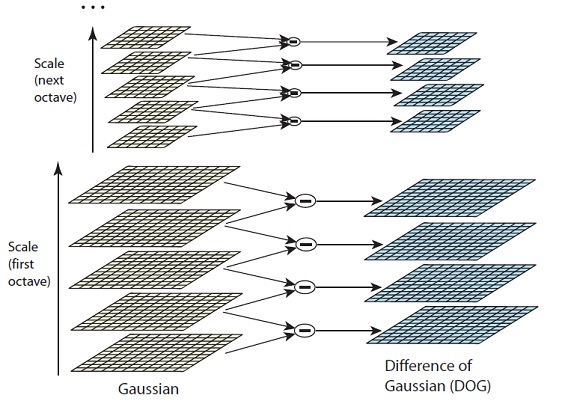
\includegraphics[width=0.90\textwidth]{fig/30.png}
     \vspace{-1em}
    \begin{center}    
       \caption{\textcolor{gray}{\footnotesize \textit{(a) Nærliggende skalabilleder for hver oktav trækkes fra og producere DoG billederne. (b) I DoG billederne udvælges ekstremaer blandt 27 nabo pixels.}}}
    \label{fig:difference}
     \end{center}
     \vspace{-2.5em}
  \end{figure} \noindent
LoG svarer til sporret af hessian matricen som angiver summen af hessian matricens egenværdier: $\nabla^2 L=\bold{tr}( \mathcal{H} )=\lambda_1+\lambda_2$. Hessian matricens egenværdier beskriver den principielle krumning i og omkring et punkt og kan derfor bruges til at udvælge forekomster af blobs. Der vil opstå et maksima når $\nabla^2 L<0$, da egenværdierne begge vil være negative og et minima når $\nabla^2 L > 0$ da egenværdierne vil være positive. Der ønskes derved at identificere ekstremaer i DoG billederne, da de vil angive forekomster af blobs. For hver pixel, sammenlignes et $3\times3\times3$ område, som vist figur \ref{fig:difference} (b). Hver pixel bliver sammenlignet med dens $8+9+9=26$ naboer i de omkringliggende DoG billeder. Et punkt udvælges som værende et ekstrema, hvis det er det største/mindste iblandt dens 26 naboer.
\\
\\
Når lokale ekstremaer er udvalgt fravælges dårligt lokaliserede punkter, f.eks. ekstremaer med lav kontrast, men også punkter, hvor ekstremaer ligger imellem pixels. Ligeledes bliver punkters placering fundet, med subpixel nøjagtighed. Dette gøres, ved non-maximal suppression, som foreslået af Lowe \cite{nonmaximalsuppression}:
\begin{equation}
D(x)=D+\dfrac{\partial D^T}{\partial x}x\dfrac{1}{2}x^T\dfrac{\partial^2D}{\partial x^2}x
\label{nonmax}
\end{equation}
Ovenstående kan forstås om en Taylor udvidelse af punket D.
Lokationen af ekstremaet $\hat{x}$ findes ved at tage den afledte af den ovenstående funktion ift. $x$ og sætte den til 0:
\begin{equation}
\hat{x}= \dfrac{\partial^2 D^{-1}}{\partial x^2}\dfrac{\partial D}{\partial x}
\label{xhat}
\end{equation}
I denne implementering er Non-maximal surpression anvendt anderledes ift. den anvendt i SIFT: Lowe foreslår, at hvis et punkt er et ekstrema, som udregnet ved ligning \ref{nonmax} og $\hat{x} > 0.5$ i en retning, skal ligning \eqref{nonmax} udregnes omkring det nye punkt og dette gentages, indtil $\hat{x} < 0.5$, eller indtil udregning er udført et max antal gange.
\\
I denne implementering bliver et punkt fjernet, hvis $\hat{x} > 0.5$ i en given retning, da dette kun vil øge antallet af interessepunkter, hvilket er vurderet til ikke at være nødvendigt, da der i forvejen lokaliseres et stort antal punkter. Det vil ligeledes øge kompleksiteten af applikationen.
\\
Punkter med lav kontrast fjernes, ved at sætte grænseværdi, for $D(\hat{x})$:
\begin{equation}
D(\hat{x})=D+\dfrac{1}{2}\dfrac{\partial D^T}{\partial x}\hat{x}
\label{dxhat}
\end{equation}
Lowe foreslår at værdier af $D(\hat{x})$ under 0.03 fjernes. Metoden vil også have en positiv respons overfor kanter, derfor anvendes metoder lånt fra Harris og Stephens \cite{harris} til at fjerne disse. Hessian matricen opstilles som:
\begin{equation}
\mathcal{H} =
\begin{bmatrix}
D_{xx} & D{xy} \\
D{xy} & D{yy}
\end{bmatrix}
\end{equation}
En negativ determinant angiver et saddle-point og fjernes derved. For at fjerne punkter lokaliseret på en kant beskrives forholdet imellem hessian matricens egenværdier, ved følgende ligning, hvor $r$ angiver størrelsesforholdet imellem egenværdierne:
\begin{equation}
\dfrac{tr(\mathcal{H})^2}{Det(\mathcal{H})}<\dfrac{(r+1)^2}{r}
\label{rval}
\end{equation}
En grænseværdi $r$ kan opstilles for at fjerne punkter lokaliseret på en kant. Punkter der tilfredsstiller denne grænseværdi udvælges som interessepunkter.
\subsection{Algoritme}
\textbf{Input:} \\
\textbf{Output:}
\begin{enumerate}
\item{Konstruer skalarummet for de forskellige oktaver, ved iterativt at folde skalabilledet med en stigende værdi af $\sigma$: $$ L(x,y,\sigma)= G(x,y,\sigma) \ast I(x,y) $$
og halver størrelsen af billedet for hver oktav.}
\item{Udregn DOG billeder, ved at tage forskellen imellem skala billederne, som i ligning \eqref{dog}.}
\item{Lokaliser ekstremaer for hvert punkt i DOG billeder, ved at sammenligne punktet med dens 26 naboer som illustreret i figur \ref{fig:difference}.}
\item{Afvis punkter der ikke er lokaliseret på ekstremaer, og ekstremaer med lav kontrast som i ligning \eqref{xhat} og \eqref{dxhat}:
\begin{equation}
\begin{split}
\texttt{indikator} = 
\begin{cases}
\texttt{fjern}& \texttt{hvis } \hat{x}>0.5 \lor |D(\hat{x})|>0.03 \lor \bold{det} \mathcal{H}<0 , \\
\texttt{behold}& \texttt{ellers}. 
\end{cases}
\end{split}
\label{maxsurp}
\end{equation}
}
\item{Fjern punkter lokaliseret på en kant ved at opstille en grænseværdi $r$ og fjern punkter der ikke opfylder denne, som i ligning \eqref{rval}.}
\end{enumerate}
\subsection{Orientering af SIFT punkter}
Formålet ved dette skridt er at tildele hvert punkt en orientering.
\\
\\
Et $16\times 16$ dataindsamlingsvindue placeres på interessepunktets skalabillede, omkring interessepunktet. For alle punkter i dataindsamlingsvinduet, er størrelsen af punkternes gradient, og deres orientering beregnet ved:
\begin{equation}
m(x,y) = \sqrt{(L(x + 1, y) - L(x - 1, y))^2 + (L(x, y + 1) - L(x, y - 1))^2} 
\label{magnitudepoint}
\end{equation}
\begin{equation}o(x,y) = tan^{-1}((L(x,y+1) - L(x,y-1))/(L(x+1, y) - L(x-1, y))) 
\label{orientationpoint}
\end{equation}
hvor $m$ er størrelsen af en gradient, og $o$ er gradientens retning. For alle punkter indenfor dataindsamlingsvinduet, udregnes ligning
\eqref{magnitudepoint}, \eqref{orientationpoint}, og danner et gradientvindue $g$ og orienteringsvindue $v$, begge vinduer af størrelse $16\times16$. Gradientvinduet skal herefter foldes med et Gaussisk filter hvor $\sigma_{Gauss} = 1.5 \cdot \sigma_{point}$, med størrelse $16\times16$. Dette udføres for at vægte gradienter nær punktet højere end punkter i udkanten af vinduet.  $\sigma_{Gauss}$ er sigmaværdien tilhørende Gaussfiltret, der foldes med gradientvinduet. $\sigma_{point}$ er sigmaværdien i $DoG$ billedet, punktet er fundet på. 
\\
\\
Der oprettes derefter et orienteringshistogram $H$, med 36 indgange. Orienteringerne angivet i $v$ skal tilføjes histogrammet, vægtet af gradientstyrken angivet i $g$. En indgang i $H$, dækker en vinkel på $10^{\circ}$. F.eks. skal alle gradienter med vinkler mellem  $0^{\circ}-10^{\circ}$, tilføjes vægtet, til $H_1$, osv. Dette resulterer i et orienteringshistogram, hvor indgangen i histogrammet, med størst værdi, bliver bearbejdet. Lowe foreslår, at alle indgange i histogrammet, der ligger indenfor 80\% af det højeste punkt, bliver nye features - dette er undladt her, for at reducere antallet af features. 
\\
Der skal nu foretages en interpolation, omkring den indgang i histogrammet, med størst værdi, for at få et mere præcist estimat af $\theta$. Toppunktet af andengradspolynomiet vil udgøre orienteringen der tildeles punktet. 
\begin{figure}[H]
    \centering
    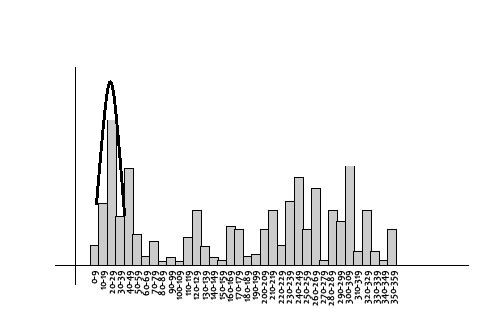
\includegraphics[width=0.60\textwidth]{fig/sift-orientation-histogram.jpg}
     \vspace{-1em}
    \begin{center}    
       \caption{{\footnotesize \textit{Histogrammet $H$ afbilledet, sammen med en andengradsligning. Andengradsligningen er beregnet over den største indgang i $H$}}}
    \label{histogramheight}
     \end{center}
     \vspace{-2.5em}
  \end{figure} \noindent
Dette ses på figur \ref{histogramheight}, hvor et andengradspolynomium er blevet tilnærmet den største værdi af $H$. Estimering af andengradspolynomiet sker over den største værdi i $H$, og dens venstre og højre nabo.


\subsubsection*{Algoritme: SIFT Orientering}
\begin{tabbing}
Input\quad \= : \= Billede $I$\\
$\text{ }$ \> : \> Interessepunkter $p  \in (x, y)$ \\
Output $\text{ }$ \> : \> Interessepunkter tildelt orientering $p \in (x,y, \theta)$
\end{tabbing}
\begin{enumerate}
\item Et dataindsamlingsvindue placeres omkring interessepunktet, på det skalabillede interessepunktet er fundet på.
\item Ligning \eqref{magnitudepoint}, \eqref{orientationpoint} anvendes på hvert punkt i dataindsamlingsvinduet, for at udregne gradient retninger og størrelser. Gradientbilledet foldes derefter med et Gaussisk filter, hvor $\sigma_{Gauss} = 1.5 \cdot \sigma_{point}$
\item Værdierne i $g$ adderes på indgange i histogrammet $H$, afhængigt af deres orientering i $v$.
\item  Der udføres en interpolation omkring den største værdi i $H$ og to naboer. Denne værdi returneres.
\end{enumerate}

\subsection{Deskriptor}
Der benyttes et datainsamlingsvindue $W$, der har størrelsen $16 \times 16$, til at indsamle information omkring et interessepunkt, og denne information udtrykkes som en vektor. Deskriptoren kan formelt beskrives:
%med 128 indgange
\\
\\
sigmaværdien i $DoG$ billedet, punktet er blevet fundet på, anvendes til videre beregning. For at opnå rotationsinvarians, bliver dataindsamlingsvinduet $W$ roteret i forhold til $\theta$, som fundet i forrige afsnit. Dette opnås, ved at tage prik produktet, af hver indgang i dataindsamlingsvinduet, med rotationsmatricen:
\begin{equation}
W_{{mn}_{new}} = W_{mn} \cdot
\begin{pmatrix}
  \cos \theta & -\sin \theta \\
  \sin \theta & \cos \theta  \\
\end{pmatrix}
\label{rotaionmatrix}
\end{equation}
$W_{{mn}_{new}}$ bruges til at indsamle information om størrelsen og orienteringen af gradienten i det $i$'ende punkt, som i ligning \eqref{magnitudepoint} og \eqref{orientationpoint} respektivt - gradienten og orienteringen bliver gemt i to separate matricer af størrelse $16\times16$, hhv $g$ og $o$. $g$ bliver herefter foldet med et Gaussisk filter størrelse $16\times16$, hvor sigmaværdien er halv så stor, som størrelsen af vinduet ($\sigma=8$):
\begin{equation}
g_{new} = G(x,y,8) * g(x,y)
\label{gradientsmooth}
\end{equation}
Herefter skal $G_{new}$ inddeles i 16 regioner ($R_{ij} \subseteq (G_{new}$), hver med størrelse $4\times4$, som set i figur(???). Der skal foretages trilineær interpolation, og alle de kontinuerte orienteringer i $O$, skal vægtes som beskrevet nedenfor, og værdierne i figur (???, b), der svarer til $F_i$, skal opdateres - her er $F_i$ repræsenteret ved 16 vinduer, hver med 8 retninger (svarede til 45 grader). Dette sker i 3 skridt:
\begin{enumerate}
\item{ alle punkter i $R_{ij}$ skal vægtes efter, hvor langt de ligger fra centrum af $R_{ij}$. Det er vedtaget, at der eksisterer tre længder (beskriv v. billede!!!)}
\item{ 4 indgange i $F_i$ opdateres efter punkterne i $R_{ij}$'s orientering. Punkterne i $R_{ij}$ skal fordeles på de 4 af de 8 orienteringer, der ligger tættest orienteringen af $R_{ij}$. Disse skal vægtes med $G_{new}$ og værdien fundet i 1. }
\item{ De 4 indgange, der er blevet opdateret, skal tilsvarende opdateres i 3 naboområder, af $F_i$ (hvis der eksisterer nogen)}
\end{enumerate}

$F$ normaliseres, og alle værdier større end 0.2 skal sættes til 0.2, og $F$ skal normaliseres igen.
\subsubsection*{Algoritme: SIFT deskriptor}
\begin{enumerate}
\item[Input:] Billede $I$.
\item[] Punkter $p \in (x, y, \theta)$
\item[Output:] En feature vektor $F$, for hver punkt $p$.
\end{enumerate}
\begin{enumerate}
\item Det bestemmes via $\sigma$ hvilket billede der skal udføres beregninger på
\item $W$ roteres, ved rotationsmatricen \eqref{rotaionmatrix}, og glattes med \eqref{gradientsmooth}
\item $R_{ij}$ oprettes, ved at dele $g_{new}$ op i 16 regioner, hver med størrelse $4\times4$
\item Alle punkter, i alle regioner af $R_{ij}$, skal nu bruges til at opdatere $F$, som beskrevet de 3 skridt ovenfor
\end{enumerate}